\section{最適解を求める問題}
\begin{frame}
\frametitle{最短経路問題}
  \begin{itemize}
\item カーナビや乗換案内や地図で所要時間の短い経路や旅費の安い経路を案内してくれるます
\item これはグラフ理論 (Graph Theory) と呼ばれる世界の最短経路問題に帰着できます
\item 与えられた条件で最適解を求めるという問題
  \end{itemize}
  \begin{block}{余裕のある人向け quiz}
    \begin{itemize}
\item 出発地と到着地がそれぞれ与えられたとしてコストが最も小さい経路を計算するプログラムを作成してください
\item $n$ 個の node を持つとして \(O(n^2)\) のオーダで計算できます
\item グラフの表現方法を変えると \(O(n\log n)\) にできます
    \end{itemize}
  \end{block}
\end{frame}
\begin{frame}
\frametitle{グラフ理論}
  \begin{itemize}
\item グラフとはあるデータ間の関係だけに注目したモデル
\item $N$ をノードの集合 (a set of nodes), $E$ をエッジの集合 (a set of edges) としてグラフ $G$ は \((N,E)\) の対である
\item 各ノードとエッジにはラベルが付けられていて,ラベルの集合を $L$ とする
  \end{itemize}
  \begin{center}
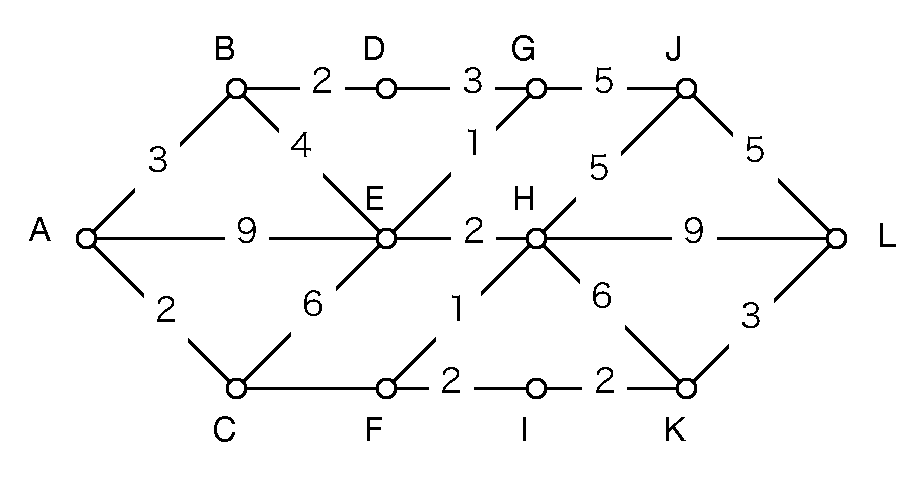
\includegraphics[scale=0.5]{./Figure/elementaryCS-2nd-figSPP.eps}
  \end{center}
\end{frame}
\begin{frame}
\frametitle{最短経路問題 (Shortest Pahts Problem)}
  \begin{itemize}
\item \(G=(N,E)\) で各エッジにコストでラベル付けし,
\item 任意の出発点が与えられたとして,他の地点に至る最小コストの経路を求める問題
  \end{itemize}
  \begin{columns}
    \begin{column}{0.3\textwidth}
      \begin{center}
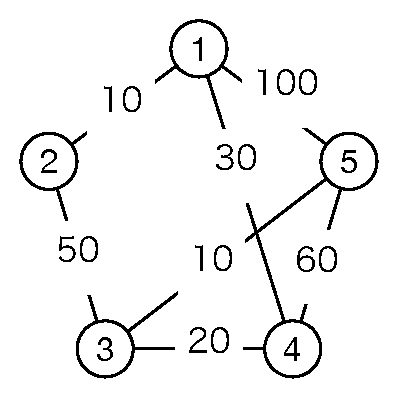
\includegraphics[scale=0.35]{./Figure/elementaryCS-2nd-figSPP-Sample.eps}
      \end{center}
    \end{column}
    \begin{column}{0.65\textwidth}
      \begin{center}
\footnotesize
        \begin{tabular}{cccccc}
S&w&D[2]&D[3]&D[4]&D[5]\\
\hline
\{1\}&\textendash&10&&30&100\\
\{1,2\}&2&10&60&30&100\\
\{1,2,4\}&4&10&50&30&90\\
\{1,2,4,3\}&3&10&50&30&60\\
\{1,2,4,3,5\}&5&10&50&30&60
        \end{tabular}
      \end{center}
    \end{column}
  \end{columns}
\end{frame}
